\documentclass[]{book}
\usepackage{lmodern}
\usepackage{amssymb,amsmath}
\usepackage{ifxetex,ifluatex}
\usepackage{fixltx2e} % provides \textsubscript
\ifnum 0\ifxetex 1\fi\ifluatex 1\fi=0 % if pdftex
  \usepackage[T1]{fontenc}
  \usepackage[utf8]{inputenc}
\else % if luatex or xelatex
  \ifxetex
    \usepackage{mathspec}
  \else
    \usepackage{fontspec}
  \fi
  \defaultfontfeatures{Ligatures=TeX,Scale=MatchLowercase}
\fi
% use upquote if available, for straight quotes in verbatim environments
\IfFileExists{upquote.sty}{\usepackage{upquote}}{}
% use microtype if available
\IfFileExists{microtype.sty}{%
\usepackage{microtype}
\UseMicrotypeSet[protrusion]{basicmath} % disable protrusion for tt fonts
}{}
\usepackage[margin=1in]{geometry}
\usepackage{hyperref}
\hypersetup{unicode=true,
            pdftitle={Linear models},
            pdfauthor={Léo Belzile},
            pdfborder={0 0 0},
            breaklinks=true}
\urlstyle{same}  % don't use monospace font for urls
\usepackage{natbib}
\bibliographystyle{apalike2}
\usepackage{color}
\usepackage{fancyvrb}
\newcommand{\VerbBar}{|}
\newcommand{\VERB}{\Verb[commandchars=\\\{\}]}
\DefineVerbatimEnvironment{Highlighting}{Verbatim}{commandchars=\\\{\}}
% Add ',fontsize=\small' for more characters per line
\usepackage{framed}
\definecolor{shadecolor}{RGB}{248,248,248}
\newenvironment{Shaded}{\begin{snugshade}}{\end{snugshade}}
\newcommand{\KeywordTok}[1]{\textcolor[rgb]{0.13,0.29,0.53}{\textbf{#1}}}
\newcommand{\DataTypeTok}[1]{\textcolor[rgb]{0.13,0.29,0.53}{#1}}
\newcommand{\DecValTok}[1]{\textcolor[rgb]{0.00,0.00,0.81}{#1}}
\newcommand{\BaseNTok}[1]{\textcolor[rgb]{0.00,0.00,0.81}{#1}}
\newcommand{\FloatTok}[1]{\textcolor[rgb]{0.00,0.00,0.81}{#1}}
\newcommand{\ConstantTok}[1]{\textcolor[rgb]{0.00,0.00,0.00}{#1}}
\newcommand{\CharTok}[1]{\textcolor[rgb]{0.31,0.60,0.02}{#1}}
\newcommand{\SpecialCharTok}[1]{\textcolor[rgb]{0.00,0.00,0.00}{#1}}
\newcommand{\StringTok}[1]{\textcolor[rgb]{0.31,0.60,0.02}{#1}}
\newcommand{\VerbatimStringTok}[1]{\textcolor[rgb]{0.31,0.60,0.02}{#1}}
\newcommand{\SpecialStringTok}[1]{\textcolor[rgb]{0.31,0.60,0.02}{#1}}
\newcommand{\ImportTok}[1]{#1}
\newcommand{\CommentTok}[1]{\textcolor[rgb]{0.56,0.35,0.01}{\textit{#1}}}
\newcommand{\DocumentationTok}[1]{\textcolor[rgb]{0.56,0.35,0.01}{\textbf{\textit{#1}}}}
\newcommand{\AnnotationTok}[1]{\textcolor[rgb]{0.56,0.35,0.01}{\textbf{\textit{#1}}}}
\newcommand{\CommentVarTok}[1]{\textcolor[rgb]{0.56,0.35,0.01}{\textbf{\textit{#1}}}}
\newcommand{\OtherTok}[1]{\textcolor[rgb]{0.56,0.35,0.01}{#1}}
\newcommand{\FunctionTok}[1]{\textcolor[rgb]{0.00,0.00,0.00}{#1}}
\newcommand{\VariableTok}[1]{\textcolor[rgb]{0.00,0.00,0.00}{#1}}
\newcommand{\ControlFlowTok}[1]{\textcolor[rgb]{0.13,0.29,0.53}{\textbf{#1}}}
\newcommand{\OperatorTok}[1]{\textcolor[rgb]{0.81,0.36,0.00}{\textbf{#1}}}
\newcommand{\BuiltInTok}[1]{#1}
\newcommand{\ExtensionTok}[1]{#1}
\newcommand{\PreprocessorTok}[1]{\textcolor[rgb]{0.56,0.35,0.01}{\textit{#1}}}
\newcommand{\AttributeTok}[1]{\textcolor[rgb]{0.77,0.63,0.00}{#1}}
\newcommand{\RegionMarkerTok}[1]{#1}
\newcommand{\InformationTok}[1]{\textcolor[rgb]{0.56,0.35,0.01}{\textbf{\textit{#1}}}}
\newcommand{\WarningTok}[1]{\textcolor[rgb]{0.56,0.35,0.01}{\textbf{\textit{#1}}}}
\newcommand{\AlertTok}[1]{\textcolor[rgb]{0.94,0.16,0.16}{#1}}
\newcommand{\ErrorTok}[1]{\textcolor[rgb]{0.64,0.00,0.00}{\textbf{#1}}}
\newcommand{\NormalTok}[1]{#1}
\usepackage{longtable,booktabs}
\usepackage{graphicx,grffile}
\makeatletter
\def\maxwidth{\ifdim\Gin@nat@width>\linewidth\linewidth\else\Gin@nat@width\fi}
\def\maxheight{\ifdim\Gin@nat@height>\textheight\textheight\else\Gin@nat@height\fi}
\makeatother
% Scale images if necessary, so that they will not overflow the page
% margins by default, and it is still possible to overwrite the defaults
% using explicit options in \includegraphics[width, height, ...]{}
\setkeys{Gin}{width=\maxwidth,height=\maxheight,keepaspectratio}
\IfFileExists{parskip.sty}{%
\usepackage{parskip}
}{% else
\setlength{\parindent}{0pt}
\setlength{\parskip}{6pt plus 2pt minus 1pt}
}
\setlength{\emergencystretch}{3em}  % prevent overfull lines
\providecommand{\tightlist}{%
  \setlength{\itemsep}{0pt}\setlength{\parskip}{0pt}}
\setcounter{secnumdepth}{5}
% Redefines (sub)paragraphs to behave more like sections
\ifx\paragraph\undefined\else
\let\oldparagraph\paragraph
\renewcommand{\paragraph}[1]{\oldparagraph{#1}\mbox{}}
\fi
\ifx\subparagraph\undefined\else
\let\oldsubparagraph\subparagraph
\renewcommand{\subparagraph}[1]{\oldsubparagraph{#1}\mbox{}}
\fi

%%% Use protect on footnotes to avoid problems with footnotes in titles
\let\rmarkdownfootnote\footnote%
\def\footnote{\protect\rmarkdownfootnote}

%%% Change title format to be more compact
\usepackage{titling}

% Create subtitle command for use in maketitle
\newcommand{\subtitle}[1]{
  \posttitle{
    \begin{center}\large#1\end{center}
    }
}

\setlength{\droptitle}{-2em}

  \title{Linear models}
    \pretitle{\vspace{\droptitle}\centering\huge}
  \posttitle{\par}
    \author{Léo Belzile}
    \preauthor{\centering\large\emph}
  \postauthor{\par}
      \predate{\centering\large\emph}
  \postdate{\par}
    \date{version of 2018-09-18}

\usepackage{booktabs}
\usepackage{amsthm}
\makeatletter
\def\thm@space@setup{%
  \thm@preskip=8pt plus 2pt minus 4pt
  \thm@postskip=\thm@preskip
}
\makeatother

\usepackage{framed,color}
\definecolor{shadecolor}{RGB}{248,248,248}

\renewcommand{\textfraction}{0.05}
\renewcommand{\topfraction}{0.8}
\renewcommand{\bottomfraction}{0.8}
\renewcommand{\floatpagefraction}{0.75}

\renewenvironment{quote}{\begin{VF}}{\end{VF}}
\let\oldhref\href
\renewcommand{\href}[2]{#2\footnote{\url{#1}}}

\ifxetex
  \usepackage{letltxmacro}
  \setlength{\XeTeXLinkMargin}{1pt}
  \LetLtxMacro\SavedIncludeGraphics\includegraphics
  \def\includegraphics#1#{% #1 catches optional stuff (star/opt. arg.)
    \IncludeGraphicsAux{#1}%
  }%
  \newcommand*{\IncludeGraphicsAux}[2]{%
    \XeTeXLinkBox{%
      \SavedIncludeGraphics#1{#2}%
    }%
  }%
\fi

\makeatletter
\newenvironment{kframe}{%
\medskip{}
\setlength{\fboxsep}{.8em}
 \def\at@end@of@kframe{}%
 \ifinner\ifhmode%
  \def\at@end@of@kframe{\end{minipage}}%
  \begin{minipage}{\columnwidth}%
 \fi\fi%
 \def\FrameCommand##1{\hskip\@totalleftmargin \hskip-\fboxsep
 \colorbox{shadecolor}{##1}\hskip-\fboxsep
     % There is no \\@totalrightmargin, so:
     \hskip-\linewidth \hskip-\@totalleftmargin \hskip\columnwidth}%
 \MakeFramed {\advance\hsize-\width
   \@totalleftmargin\z@ \linewidth\hsize
   \@setminipage}}%
 {\par\unskip\endMakeFramed%
 \at@end@of@kframe}
\makeatother

\makeatletter
\@ifundefined{Shaded}{
}{\renewenvironment{Shaded}{\begin{kframe}}{\end{kframe}}}
\makeatother

\newenvironment{rmdblock}[1]
  {
  \begin{itemize}
  \renewcommand{\labelitemi}{
    \raisebox{-.7\height}[0pt][0pt]{
      {\setkeys{Gin}{width=3em,keepaspectratio}\includegraphics{images/#1}}
    }
  }
  \setlength{\fboxsep}{1em}
  \begin{kframe}
  \item
  }
  {
  \end{kframe}
  \end{itemize}
  }
\newenvironment{rmdnote}
  {\begin{rmdblock}{note}}
  {\end{rmdblock}}
\newenvironment{rmdcaution}
  {\begin{rmdblock}{caution}}
  {\end{rmdblock}}
\newenvironment{rmdimportant}
  {\begin{rmdblock}{important}}
  {\end{rmdblock}}
\newenvironment{rmdtip}
  {\begin{rmdblock}{tip}}
  {\end{rmdblock}}
\newenvironment{rmdwarning}
  {\begin{rmdblock}{warning}}
  {\end{rmdblock}}

\let\BeginKnitrBlock\begin \let\EndKnitrBlock\end
\begin{document}
\maketitle

{
\setcounter{tocdepth}{1}
\tableofcontents
}
\chapter*{Preliminary remarks}\label{preliminary-remarks}
\addcontentsline{toc}{chapter}{Preliminary remarks}

This is a web complement to MATH 341 (Linear Models), a first regression
course for EPFL mathematicians.

We shall use the \textbf{R} programming language througout the course
(as it is free and it is used in other statistics courses at EPFL).
Visit \href{https://cran.r-project.org/}{the R-project website} to
download the program. The most popular graphical cross-platform
front-end is
\href{https://www.rstudio.com/products/rstudio/download/}{RStudio
Desktop}.

\textbf{R} is an object-oriented interpreted language. It differs from
usual programming languages in that it is designed for interactive
analyses.

Since \textbf{R} is not a conventional programming language, my teaching
approach will be learning-by-doing. The benefit of using
\emph{Rmarkdown} is that you see the output directly and you can also
copy the code.

\chapter{Introduction}\label{introduction}

You can find several introductions to \textbf{R} online. Have a look at
the \href{https://cran.r-project.org/manuals.html}{\textbf{R} manuals}
or better at
\href{https://cran.r-project.org/other-docs.html}{contributed manuals}.
A nice official reference is
\href{http://colinfay.me/intro-to-r/index.html}{An introduction to
\textbf{R}}. You may wish to look up the following chapters of the
\textbf{R} language definition
(\href{http://colinfay.me/r-language-definition/evaluation-of-expressions.html}{Evaluation
of expressions} and part of the
\href{http://colinfay.me/r-language-definition/objects.html}{\emph{Objects}
chapter}).

\section{\texorpdfstring{Basics of
\textbf{R}}{Basics of R}}\label{basics-of-r}

\subsection{Help}\label{help}

Help can be accessed via \texttt{help} or simply \texttt{?}. If you do
not know what to query, use \texttt{??} in front of a string, delimited
by captions \texttt{"\ "} as in \texttt{??"Cholesky\ decomposition"}.
Help is your best friend if you don't know what a function does, what
are its arguments, etc.

\subsection{Basic commands}\label{basic-commands}

Basic \textbf{R} commands are fairly intuitive, especially if you want
to use your \textbf{R} as a calculator. Elementary functions such as
\texttt{sum}, \texttt{min}, \texttt{max}, \texttt{sqrt}, \texttt{log},
\texttt{exp}, etc., are self-explanatory.

\begin{itemize}
\tightlist
\item
  Use \texttt{\textless{}-} to assign to a variable, and \texttt{=} for
  matching arguments inside functions
\item
  Indexing in \textbf{R} starts at 1, \textbf{not} zero.
\item
  Most functions in \textbf{R} are vectorized, so avoid loops as much as
  possible.
\item
  Integers are obtained by appending \texttt{L} to the number, so
  \texttt{2L} is an integer and \texttt{2} a double.
\end{itemize}

Besides integers and doubles, the common types are - logicals
(\texttt{TRUE} and \texttt{FALSE}); - null pointers (\texttt{NULL}),
which can be assigned to arguments; - missing values, namely \texttt{NA}
or \texttt{NaN}. These can also be obtained a result of invalid
mathematical operations such as \texttt{log(-2)}.

The above illustrates a caveat of \textbf{R}: invalid calls will often
returns \emph{something} rather than an error. It is therefore good
practice to check that the output is sensical.

\subsection{\texorpdfstring{Linear algebra in
\textbf{R}}{Linear algebra in R}}\label{linear-algebra-in-r}

\textbf{R} is an object oriented language, and the basic elements in
\textbf{R} are (column) vector. Below is a glossary with some useful
commands for performing basic manipulation of vectors and matrix
operations:

\begin{itemize}
\tightlist
\item
  \texttt{c} creates a vector
\item
  \texttt{cbind} (\texttt{rbind}) binds column (row) vectors
\item
  \texttt{matrix} and \texttt{vector} are constructors
\item
  \texttt{diag} creates a diagonal matrix (by default with ones)
\item
  \texttt{t} is the function for transpose
\item
  \texttt{solve} performs matrix inversion
\item
  \texttt{\%*\%} is matrix multiplication, \texttt{*} is element-wise
  multiplication
\item
  \texttt{crossprod} \texttt{crossprod(A,\ B)} calculates the
  cross-product, \texttt{t(A)\ \%*\%\ B} of two matrices \texttt{A} and
  \texttt{B}
\item
  \texttt{eigen}/\texttt{chol}/\texttt{qr} perform respectively an
  eigendecomposition/Cholesky/QR decomposition of a matrix
\item
  \texttt{rep} creates a vector of duplicates, \texttt{seq} a sequence.
  For integers \(i\), \(j\) with \(i<j\), \texttt{i:j} generates the
  sequence \(i, i+1, \ldots, j-1, j\).
\end{itemize}

Subsetting is fairly intuitive and general; you can use vectors, logical
statements. For example, if \texttt{x} is a vector, then

\begin{itemize}
\tightlist
\item
  \texttt{x{[}2{]}} returns the second element
\item
  \texttt{x{[}-2{]}} returns all but the second element
\item
  \texttt{x{[}1:5{]}} returns the first five elements
\item
  \texttt{x{[}(length(x)\ -\ 5):length(x){]}} returns the last five
  elements
\item
  \texttt{x{[}c(1,\ 2,\ 4){]}} returns the first, second and fourth
  element
\item
  \texttt{x{[}x\ \textgreater{}\ 3{]}} return any element greater than
  3. Possibly an empty vector of length zero!
\item
  \texttt{x{[}\ x\ \textless{}\ -2\ \textbar{}\ x\ \textgreater{}\ 2{]}}
  multiple logical conditions.
\item
  \texttt{which(x\ ==\ max(x))} index of elements satisfying a logical
  condition.
\end{itemize}

For a matrix \texttt{x}, subsetting now involves dimensions:
\texttt{{[}1,2{]}} returns the element in the first row, second column.
\texttt{x{[},2{]}} will return all of the rows, but only the second
column. For lists, you can use \texttt{{[}{[}} for subsetting by index
or the \texttt{\$} sign by names.

\subsection{Packages}\label{packages}

The great strength of \textbf{R} comes from its contributed libraries
(called packages), which contain functions and datasets provided by
third parties. Some of these (\texttt{base}, \texttt{stats},
\texttt{graphics}, etc.) are loaded by default whenever you open a
session.

To install a package from CRAN, use
\texttt{install.packages("package")}, replacing \texttt{package} by the
package name. Once installed, packages can be loaded using
\texttt{library(package)}; all the functions in \texttt{package} will be
available in the environment.

\BeginKnitrBlock{rmdcaution}
The drawback of loading packages is that, if a function with the same
name from another package is already present in your environment, it
will be hidden. To palliate to this, you can use the \texttt{::} syntax
to access a single function from an installed package, following the
model \texttt{package::function}.
\EndKnitrBlock{rmdcaution}

\section{Tutorial 1}\label{week1}

\subsection{Data sets}\label{data-sets}

We start by loading a dataset of the Old Faithful Geyser of Yellowstone
National park.

\begin{itemize}
\tightlist
\item
  Data sets are typically stored inside a \texttt{data.frame}, a
  matrix-like object whose columns contain the variables and the rows
  the observation vectors.
\item
  The columns can be of different types (\texttt{integer},
  \texttt{double}, \texttt{logical}, \texttt{character}), but all the
  column vectors must be of the same length.
\item
  Variable names can be displayed by using \texttt{names(faithful)}.
\item
  Individual columns can be accessed using the column name using the
  \texttt{\$} operator. For example, \texttt{faithful\$eruptions} will
  return the first column of the \texttt{faithful} dataset.
\item
  To load a package already present in an \textbf{R} package, use the
  command \texttt{data} with the name of the \texttt{package} as an
  argument (must be a string).
\end{itemize}

The following functions can be useful to get a quick glimpse of the
data:

\begin{itemize}
\tightlist
\item
  \texttt{summary} provides descriptive statistics for the variable.
\item
  \texttt{str} provides the first few elements with each variable, along
  with the dimension
\item
  \texttt{head} (\texttt{tail}) prints the first (last) \(n\) lines of
  the object to the console (default is \(n=6\)).
\end{itemize}

\begin{Shaded}
\begin{Highlighting}[]
\CommentTok{# Load Old faithful dataset}
\KeywordTok{data}\NormalTok{(faithful, }\DataTypeTok{package =} \StringTok{"datasets"}\NormalTok{)}
\CommentTok{# Query the database for documentation}
\NormalTok{?faithful}
\CommentTok{# look at first entries}
\KeywordTok{head}\NormalTok{(faithful)}
\end{Highlighting}
\end{Shaded}

\begin{verbatim}
##   eruptions waiting
## 1     3.600      79
## 2     1.800      54
## 3     3.333      74
## 4     2.283      62
## 5     4.533      85
## 6     2.883      55
\end{verbatim}

\begin{Shaded}
\begin{Highlighting}[]
\KeywordTok{str}\NormalTok{(faithful)}
\end{Highlighting}
\end{Shaded}

\begin{verbatim}
## 'data.frame':    272 obs. of  2 variables:
##  $ eruptions: num  3.6 1.8 3.33 2.28 4.53 ...
##  $ waiting  : num  79 54 74 62 85 55 88 85 51 85 ...
\end{verbatim}

\begin{Shaded}
\begin{Highlighting}[]
\CommentTok{# What kind of object is faithful? }
\KeywordTok{class}\NormalTok{(faithful)}
\end{Highlighting}
\end{Shaded}

\begin{verbatim}
## [1] "data.frame"
\end{verbatim}

Other common classes are \texttt{matrix} and \texttt{list}. The former
has attributes \texttt{dim}, \texttt{ncol} and \texttt{nrow} in addition
to \texttt{length}, which gives the total number of elements. A
\texttt{list} is an unstructured class whose elements are accessed using
double indexing \texttt{{[}{[}\ {]}{]}} and elements are typically
accessed using \texttt{\$} symbol with names. To delete an element from
a list, assign \texttt{NULL} to it. \texttt{data.frame} is a special
type of list where all the elements are vectors of potentially different
type, but of the same length.

\subsection{Graphics}\label{graphics}

The \texttt{faithful} dataset consists of two variables: the regressand
\texttt{waiting} and the regressor \texttt{eruptions}. One could
postulate that the waiting time between eruptions will be smaller if the
eruption time is small, since pressure needs to build up for the
eruption to happen. We can look at the data to see if there is a linear
relationship between the variables.

An image is worth a thousand words and in statistics, visualization is
crucial. Scatterplots are produced using the function \texttt{plot}. You
can control the graphic console options using \texttt{par} --- see
\texttt{?plot} and \texttt{?par} for a description of the basic and
advanced options available.

Once \texttt{plot} has been called, you can add additional observations
as points (lines) to the graph using \texttt{point} (\texttt{lines}) in
place of \texttt{plot}. If you want to add a line (horizontal, vertical,
or with known intercept and slope), use the function \texttt{abline}.

Other functions worth mentioning at this stage:

\begin{itemize}
\tightlist
\item
  \texttt{boxplot} creates a box-and-whiskers plot
\item
  \texttt{hist} creates an histogram, either on frequency or probability
  scale (option \texttt{freq\ =\ FALSE}). \texttt{breaks} control the
  number of bins. \texttt{rug} adds lines below the graph indicating the
  value of the observations.
\item
  \texttt{pairs} creates a matrix of scatterplots, akin to \texttt{plot}
  for data frame objects.
\end{itemize}

\BeginKnitrBlock{rmdnote}
There are two options for basic graphics: the base graphics package and
the package \texttt{ggplot2}. The latter is a more recent proposal that
builds on a modular approach and is more easily customizable --- I
suggest you stick to either and \texttt{ggplot2} is a good option if you
don't know \textbf{R} already, as the learning curve will be about the
same. Even if the display from \texttt{ggplot2} is nicer, this is no
excuse for not making proper graphics. Always label the axis and include
measurement units!
\EndKnitrBlock{rmdnote}

\begin{Shaded}
\begin{Highlighting}[]
\CommentTok{# Scatterplots}
\CommentTok{# Using default R commands}
\KeywordTok{plot}\NormalTok{(waiting }\OperatorTok{~}\StringTok{ }\NormalTok{eruptions, }\DataTypeTok{data =}\NormalTok{ faithful, }
     \DataTypeTok{xlab =} \StringTok{"Eruption time (in min.)"}\NormalTok{, }
     \DataTypeTok{ylab =} \StringTok{"Waiting time between eruptions (in min.)"}\NormalTok{,}
     \DataTypeTok{main =} \StringTok{"Old Faithful Geyser Data"}\NormalTok{)}
\end{Highlighting}
\end{Shaded}

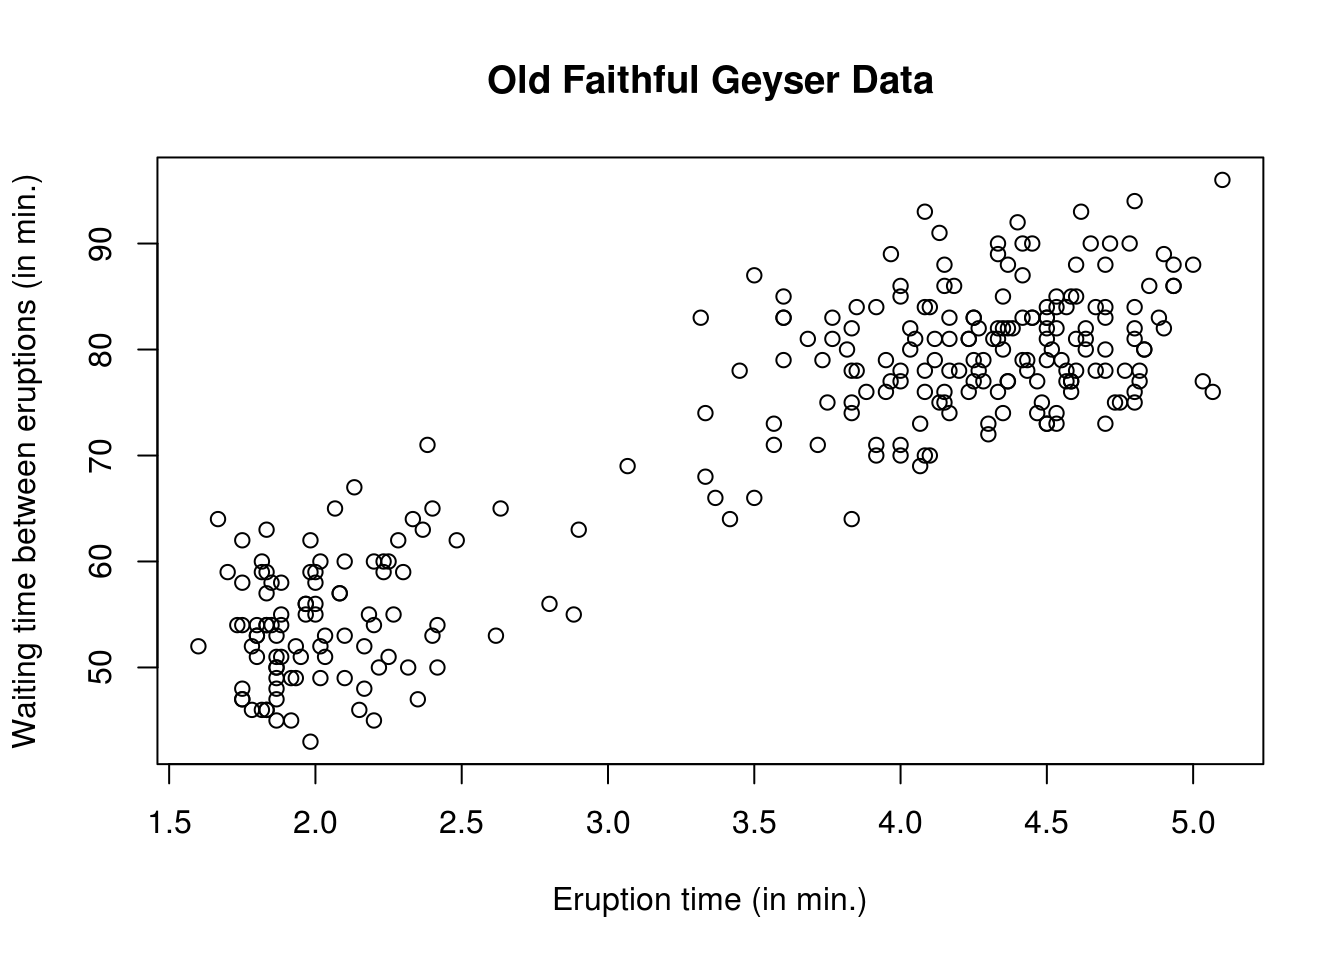
\includegraphics{LinesRModels_files/figure-latex/week1_scatterplot-1.pdf}

\begin{Shaded}
\begin{Highlighting}[]
\CommentTok{#using the grammar of graphics (more modular)}
\CommentTok{#install.packages("ggplot2") #do this once only}
\KeywordTok{library}\NormalTok{(ggplot2)}
\NormalTok{ggplot2}\OperatorTok{::}\KeywordTok{ggplot}\NormalTok{(}\DataTypeTok{data =}\NormalTok{ faithful, }\KeywordTok{aes}\NormalTok{(}\DataTypeTok{x =}\NormalTok{ eruptions, }\DataTypeTok{y =}\NormalTok{ waiting)) }\OperatorTok{+}\StringTok{ }
\StringTok{  }\KeywordTok{geom_point}\NormalTok{() }\OperatorTok{+}\StringTok{  }
\StringTok{  }\KeywordTok{labs}\NormalTok{(}\DataTypeTok{title =} \StringTok{"Old Faithful Geyser Data"}\NormalTok{, }
       \DataTypeTok{x =} \StringTok{"Eruption time (in min.)"}\NormalTok{, }
       \DataTypeTok{y =} \StringTok{"Waiting time between eruptions (in min.)"}\NormalTok{)}
\end{Highlighting}
\end{Shaded}

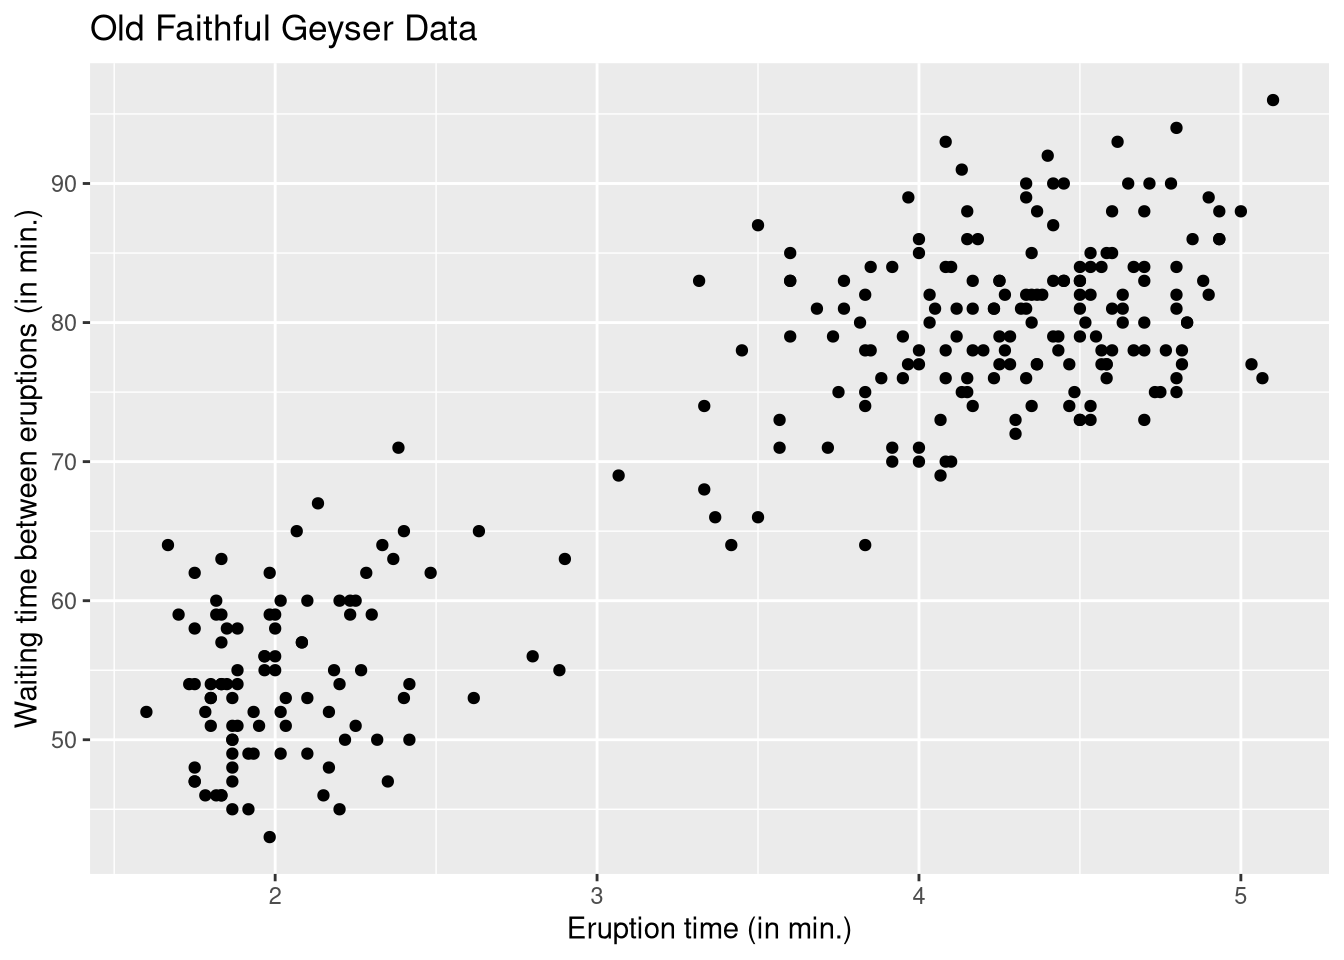
\includegraphics{LinesRModels_files/figure-latex/week1_scatterplot-2.pdf}

A simple linear model of the form
\[y_i = \beta_0 + \beta_1 \mathrm{x}_i + \varepsilon_i,\] where
\(\varepsilon_i\) is a noise variable with expectation zero and
\(\mathbf{x} = \mathsf{eruptions}\) and
\(\boldsymbol{y} = \mathsf{waiting}\). We first create a matrix with a
column of \(\mathbf{1}_n\) for the intercept. We bind vectors by column
(\texttt{cbind}) into a matrix, recycling arguments if necessary. Use
\texttt{\$} to obtain a column of the data frame based on the name of
the variable (partial matching is allowed, e.g., \texttt{faithful\$er}
is equivalent to \texttt{faithful\$eruptions} in this case).

\begin{Shaded}
\begin{Highlighting}[]
\NormalTok{## Manipulating matrices}
\NormalTok{n <-}\StringTok{ }\KeywordTok{nrow}\NormalTok{(faithful)}
\NormalTok{p <-}\StringTok{ }\KeywordTok{ncol}\NormalTok{(faithful)}
\NormalTok{y <-}\StringTok{ }\NormalTok{faithful}\OperatorTok{$}\NormalTok{waiting}
\NormalTok{X <-}\StringTok{ }\KeywordTok{cbind}\NormalTok{(}\DecValTok{1}\NormalTok{, faithful}\OperatorTok{$}\NormalTok{eruptions)}
\end{Highlighting}
\end{Shaded}

\subsection{Projection matrices}\label{projection-matrices}

Recall that
\(\mathbf{H}_{\mathbf{X}} \equiv \mathbf{X}(\mathbf{X}^\top\mathbf{X})^{-1}\mathbf{X}^\top\)
is the orthogonal projection matrix onto \(\mathsf{span}(\mathbf{X})\).
The latter has \(p=2\) eigenvalues equal to 1, is an \(n \times n\)
matrix of rank \(p\), is symmetric and idempotent. We can verify the
properties of \(\mathbf{H}_{\mathbf{X}}\) numerically.

\BeginKnitrBlock{rmdcaution}
Whereas we will frequently use \texttt{==} to check for equality of
booleans, the latter should be avoided for comparisons because computer
arithmetic is exact only in base 2. For example,
\texttt{1/10\ +\ 2/10\ -\ 3/10\ ==\ 0} will return \texttt{FALSE},
whereas \texttt{all.equal(1/10\ +\ 2/10\ -\ 3/10,\ 0)} will return
\texttt{TRUE}. Us \texttt{all.equal} to check for equalities.
\EndKnitrBlock{rmdcaution}

\begin{Shaded}
\begin{Highlighting}[]
\NormalTok{Hx <-}\StringTok{ }\NormalTok{X }\OperatorTok\StringTok{ }\KeywordTok{solve}\NormalTok{(}\KeywordTok{crossprod}\NormalTok{(X)) }\OperatorTok\StringTok{ }\KeywordTok{t}\NormalTok{(X)}
\CommentTok{# Create projection matrix onto complement }
\CommentTok{# `diag(n)` is the n by n identity matrix}
\NormalTok{Mx <-}\StringTok{ }\KeywordTok{diag}\NormalTok{(n) }\OperatorTok{-}\StringTok{ }\NormalTok{Hx}
\CommentTok{#Check that projection leaves X invariant}
\KeywordTok{isTRUE}\NormalTok{(}\KeywordTok{all.equal}\NormalTok{(X, Hx }\OperatorTok\StringTok{ }\NormalTok{X))}
\end{Highlighting}
\end{Shaded}

\begin{verbatim}
## [1] TRUE
\end{verbatim}

\begin{Shaded}
\begin{Highlighting}[]
\CommentTok{#Check that orthogonal projection maps X to zero matrix of dimension (n, p)}
\KeywordTok{isTRUE}\NormalTok{(}\KeywordTok{all.equal}\NormalTok{(}\KeywordTok{matrix}\NormalTok{(}\DecValTok{0}\NormalTok{, }\DataTypeTok{nrow =}\NormalTok{ n, }\DataTypeTok{ncol =}\NormalTok{ p), Mx }\OperatorTok\StringTok{ }\NormalTok{X))}
\end{Highlighting}
\end{Shaded}

\begin{verbatim}
## [1] TRUE
\end{verbatim}

\begin{Shaded}
\begin{Highlighting}[]
\CommentTok{#Check that the matrix Hx is idempotent}
\KeywordTok{isTRUE}\NormalTok{(}\KeywordTok{all.equal}\NormalTok{(Hx }\OperatorTok\StringTok{ }\NormalTok{Hx, Hx))}
\end{Highlighting}
\end{Shaded}

\begin{verbatim}
## [1] TRUE
\end{verbatim}

\begin{Shaded}
\begin{Highlighting}[]
\CommentTok{#Check that the matrix Hx is symmetric}
\KeywordTok{isTRUE}\NormalTok{(}\KeywordTok{all.equal}\NormalTok{(}\KeywordTok{t}\NormalTok{(Hx), Hx))}
\end{Highlighting}
\end{Shaded}

\begin{verbatim}
## [1] TRUE
\end{verbatim}

\begin{Shaded}
\begin{Highlighting}[]
\CommentTok{#Check that only a two eigenvalue are 1 and the rest are zero}
\KeywordTok{isTRUE}\NormalTok{(}\KeywordTok{all.equal}\NormalTok{(}\KeywordTok{eigen}\NormalTok{(Hx, }\DataTypeTok{only.values =} \OtherTok{TRUE}\NormalTok{)}\OperatorTok{$}\NormalTok{values, }\KeywordTok{c}\NormalTok{(}\KeywordTok{rep}\NormalTok{(}\DecValTok{1}\NormalTok{, p), }\KeywordTok{rep}\NormalTok{(}\DecValTok{0}\NormalTok{, n }\OperatorTok{-}\StringTok{ }\NormalTok{p))))}
\end{Highlighting}
\end{Shaded}

\begin{verbatim}
## [1] TRUE
\end{verbatim}

\begin{Shaded}
\begin{Highlighting}[]
\CommentTok{#Check that the matrix has rank p}
\KeywordTok{isTRUE}\NormalTok{(}\KeywordTok{all.equal}\NormalTok{(Matrix}\OperatorTok{::}\KeywordTok{rankMatrix}\NormalTok{(Hx), p, }\DataTypeTok{check.attributes =} \OtherTok{FALSE}\NormalTok{))}
\end{Highlighting}
\end{Shaded}

\begin{verbatim}
## [1] TRUE
\end{verbatim}

\subsection{Your turn}\label{your-turn}

\begin{itemize}
\tightlist
\item
  Install the \textbf{R} package \texttt{ISLR} and load the dataset
  \texttt{Auto}. Be careful, as \textbf{R} is case-sensitive.
\item
  Query the help file for information about the data set.
\item
  Look at the first lines of \texttt{Auto}
\item
  Create an explanatory variable \texttt{x} with horsepower and mileage
  per gallon as response \texttt{y}.
\item
  Create a scatterplot of \texttt{y} against \texttt{x}. Is there a
  linear relationship between the two variables?
\item
  Append a vector of ones to \texttt{x} and create a projection matrix.
\item
  Check that the resulting projection matrix is symmetric and
  idempotent.
\end{itemize}

\section{Exercises}\label{exercises}

\subsection*{(1.4) Oblique projections}\label{oblique-projections}
\addcontentsline{toc}{subsection}{(1.4) Oblique projections}

Suppose that
\(\dim(\mathsf{span}(\mathbf{X})) \neq \dim(\mathsf{span}(\mathbf{W}))\).
An oblique projection matrix is of the form
\(\mathbf{P}\equiv\mathbf{X}(\mathbf{W}^\top\mathbf{X})^{-1}\mathbf{W}^\top\)
and appears in instrumental variable regression. The oblique projection
is such that \(\mathrm{im}(\mathbf{P})=\mathsf{span}(\mathbf{X})\), but
\(\mathrm{im}(\mathbf{I}-\mathbf{P})=\mathsf{span}(\mathbf{W}^\perp)\).
This fact is illustrated below.

We consider two non-parallel vectors in \(\mathbb{R}^2\), \(\mathbf{X}\)
and \(\mathbf{W}\). The figure shows the projection of a third vector
(non-parallel to \(\mathbf{X}\) or \(\mathbf{W}\)) onto the span of
\(\mathbf{P}\) (blue), \(\mathbf{P}^\top\) (red),
\(\mathbf{I}_2-\mathbf{P}\) (dashed blue) and
\(\mathbf{I}_2-\mathbf{P}^\top\) (dashed red). The circles indicate the
points \(\mathbf{W}\) (red) and \(\mathbf{X}\) (blue) on the plane.
Notice that \(\mathbf{I}_2-\mathbf{P}^\top \perp \mathbf{P}\), whereas
\(\mathbf{I}_2-\mathbf{P} \perp \mathbf{P}^\top\).

\begin{Shaded}
\begin{Highlighting}[]
\CommentTok{#Create two vectors (non-parallel)}
\NormalTok{x <-}\StringTok{ }\KeywordTok{c}\NormalTok{(}\DecValTok{1}\NormalTok{, }\DecValTok{2}\NormalTok{)}
\NormalTok{w <-}\StringTok{ }\KeywordTok{c}\NormalTok{(}\OperatorTok{-}\DecValTok{1}\NormalTok{, }\FloatTok{0.1}\NormalTok{)}
\CommentTok{#Create oblique projection matrix}
\NormalTok{P <-}\StringTok{ }\NormalTok{x }\OperatorTok\StringTok{ }\KeywordTok{solve}\NormalTok{(}\KeywordTok{t}\NormalTok{(w) }\OperatorTok\StringTok{ }\NormalTok{x) }\OperatorTok\StringTok{ }\KeywordTok{t}\NormalTok{(w)}

\KeywordTok{isTRUE}\NormalTok{(}\KeywordTok{all.equal}\NormalTok{((P }\OperatorTok\StringTok{ }\NormalTok{P), P)) }\CommentTok{#P is idempotent}
\end{Highlighting}
\end{Shaded}

\begin{verbatim}
## [1] TRUE
\end{verbatim}

\begin{Shaded}
\begin{Highlighting}[]
\NormalTok{P }\OperatorTok{-}\StringTok{ }\KeywordTok{t}\NormalTok{(P) }\CommentTok{#but not symmetric}
\end{Highlighting}
\end{Shaded}

\begin{verbatim}
##       [,1]   [,2]
## [1,] 0.000 -2.625
## [2,] 2.625  0.000
\end{verbatim}

\begin{Shaded}
\begin{Highlighting}[]
\CommentTok{#Project a third vector `vec' onto P, P transpose, I-P, I-(P transpose)}
\NormalTok{vec <-}\StringTok{ }\KeywordTok{c}\NormalTok{(}\FloatTok{1.9}\NormalTok{, }\OperatorTok{-}\FloatTok{1.5}\NormalTok{)}
\NormalTok{vec_P <-}\StringTok{ }\NormalTok{P }\OperatorTok\StringTok{ }\NormalTok{vec}
\NormalTok{vec_Pt <-}\StringTok{ }\KeywordTok{t}\NormalTok{(P) }\OperatorTok\StringTok{ }\NormalTok{vec}
\NormalTok{vec_Id_minus_P <-}\StringTok{ }\NormalTok{(}\KeywordTok{diag}\NormalTok{(}\DecValTok{2}\NormalTok{)}\OperatorTok{-}\NormalTok{P) }\OperatorTok\StringTok{ }\NormalTok{vec }
\CommentTok{#diag: diagonal matrix, default to identity}
\NormalTok{vec_Id_minus_Pt <-}\StringTok{ }\NormalTok{(}\KeywordTok{diag}\NormalTok{(}\DecValTok{2}\NormalTok{)}\OperatorTok{-}\KeywordTok{t}\NormalTok{(P)) }\OperatorTok\StringTok{ }\NormalTok{vec}

\CommentTok{#Plot the resulting vector along with the two vectors x and w (points)}
\KeywordTok{par}\NormalTok{(}\DataTypeTok{pty =} \StringTok{"s"}\NormalTok{) }\CommentTok{#graphical console parameters (square region)}
\KeywordTok{plot}\NormalTok{(}\OtherTok{NULL}\NormalTok{, }\DataTypeTok{xlab =} \StringTok{"x"}\NormalTok{, }\DataTypeTok{ylab =} \StringTok{"y"}\NormalTok{, }\DataTypeTok{xlim =} \KeywordTok{c}\NormalTok{(}\OperatorTok{-}\DecValTok{4}\NormalTok{, }\DecValTok{4}\NormalTok{), }\DataTypeTok{ylim =} \KeywordTok{c}\NormalTok{(}\OperatorTok{-}\DecValTok{4}\NormalTok{, }\DecValTok{4}\NormalTok{))}
\CommentTok{#create empty plot with labels x and y, on square region [-4,4]^2}
\KeywordTok{points}\NormalTok{(}\DecValTok{0}\NormalTok{, }\DecValTok{0}\NormalTok{, }\DataTypeTok{pch =} \DecValTok{20}\NormalTok{) }\CommentTok{#points: add points to existing plot}
\KeywordTok{points}\NormalTok{(x[}\DecValTok{1}\NormalTok{], x[}\DecValTok{2}\NormalTok{], }\DataTypeTok{col =} \StringTok{"blue"}\NormalTok{)}
\KeywordTok{points}\NormalTok{(w[}\DecValTok{1}\NormalTok{], w[}\DecValTok{2}\NormalTok{], }\DataTypeTok{col =} \StringTok{"red"}\NormalTok{)}
\CommentTok{# blue line for P, dashed blue for I-P, red for Pt, red dashed for I-Pt}
\KeywordTok{segments}\NormalTok{(}\DataTypeTok{x0 =} \DecValTok{0}\NormalTok{, }\DataTypeTok{y0 =} \DecValTok{0}\NormalTok{, }\DataTypeTok{x1 =}\NormalTok{ vec_P[}\DecValTok{1}\NormalTok{], }\DataTypeTok{y1 =}\NormalTok{ vec_P[}\DecValTok{2}\NormalTok{], }\DataTypeTok{col =} \StringTok{"blue"}\NormalTok{)}
\KeywordTok{segments}\NormalTok{(}\DataTypeTok{x0 =} \DecValTok{0}\NormalTok{, }\DataTypeTok{y0 =} \DecValTok{0}\NormalTok{, }\DataTypeTok{x1 =}\NormalTok{ vec_Pt[}\DecValTok{1}\NormalTok{], }\DataTypeTok{y1 =}\NormalTok{ vec_Pt[}\DecValTok{2}\NormalTok{], }\DataTypeTok{col =} \StringTok{"red"}\NormalTok{)}
\KeywordTok{segments}\NormalTok{(}\DataTypeTok{x0 =} \DecValTok{0}\NormalTok{, }\DataTypeTok{y0 =} \DecValTok{0}\NormalTok{, }\DataTypeTok{x1 =}\NormalTok{ vec_Id_minus_P[}\DecValTok{1}\NormalTok{], }\DataTypeTok{y1 =}\NormalTok{ vec_Id_minus_P[}\DecValTok{2}\NormalTok{], }\DataTypeTok{col =} \StringTok{"blue"}\NormalTok{, }\DataTypeTok{lty =} \DecValTok{2}\NormalTok{)}
\KeywordTok{segments}\NormalTok{(}\DataTypeTok{x0 =} \DecValTok{0}\NormalTok{, }\DataTypeTok{y0 =} \DecValTok{0}\NormalTok{, }\DataTypeTok{x1 =}\NormalTok{ vec_Id_minus_Pt[}\DecValTok{1}\NormalTok{], }\DataTypeTok{y1 =}\NormalTok{ vec_Id_minus_Pt[}\DecValTok{2}\NormalTok{], }\DataTypeTok{col =} \StringTok{"red"}\NormalTok{, }\DataTypeTok{lty =} \DecValTok{2}\NormalTok{)}
\end{Highlighting}
\end{Shaded}

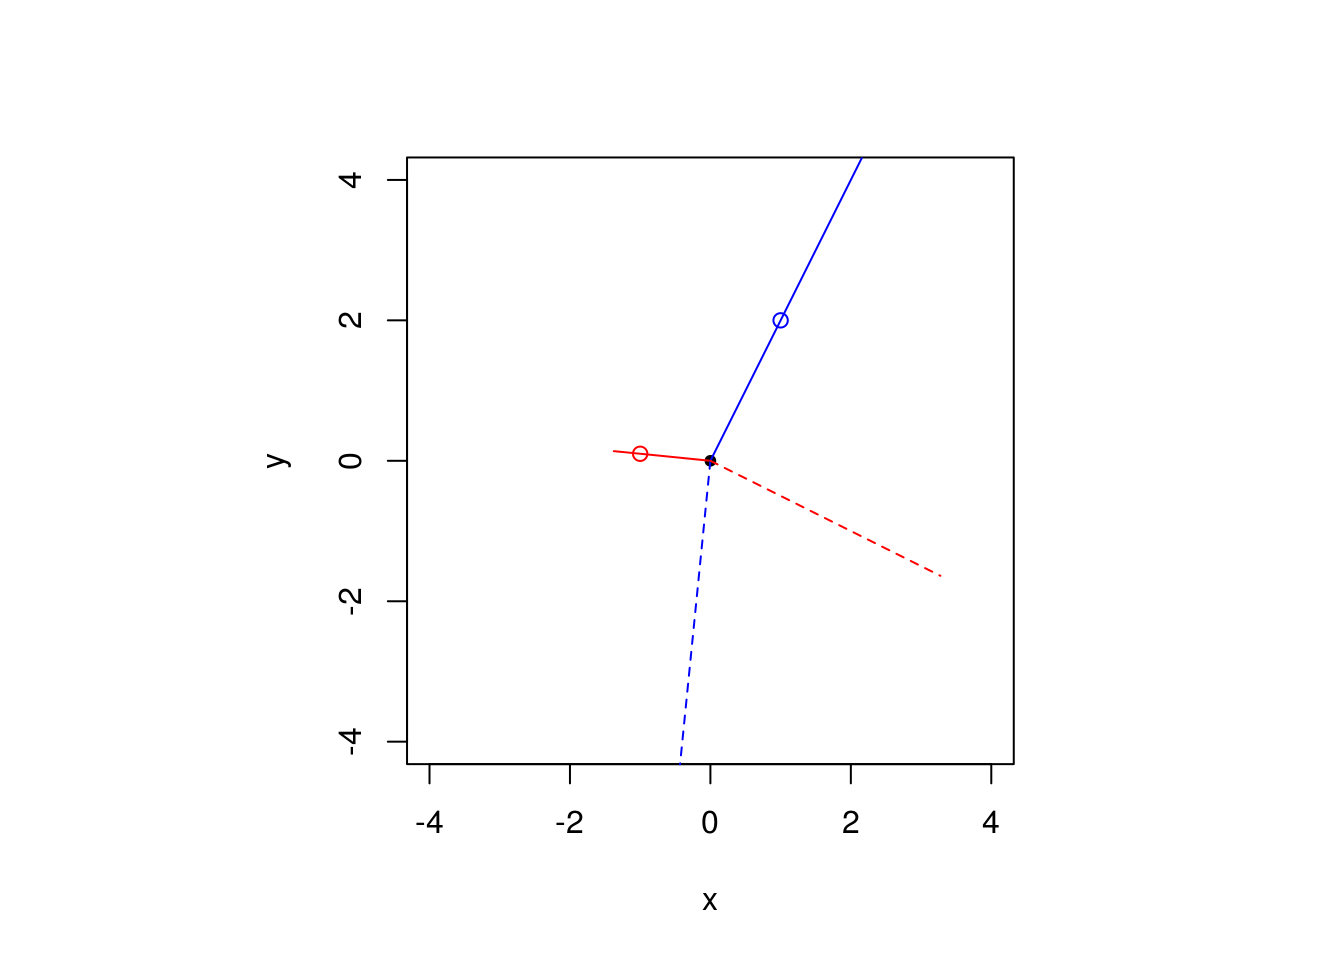
\includegraphics{LinesRModels_files/figure-latex/oblique_projection-1.pdf}

\bibliography{book.bib,packages.bib}


\end{document}
